\documentclass[conference]{IEEEtran}
\IEEEoverridecommandlockouts

% ==============================================================================
% Packages
% ==============================================================================
\usepackage[utf8]{inputenc}
\usepackage[T1]{fontenc}
\usepackage{cite}
\usepackage{amsmath, amssymb, amsfonts}
\usepackage{algorithm}
\usepackage{algorithmic}
\usepackage{graphicx}
\usepackage{textcomp}
\usepackage{xcolor}
\usepackage{booktabs}
\usepackage{tabularx}
\usepackage{multirow}
\usepackage{subcaption}
\usepackage{url}
\usepackage{microtype}

\graphicspath{{images/}}

\begin{document}

\title{Optimizing IDS Rule Placement via Set Covering with Capacity Constraints: A Multi-Sensor Attack Graph Approach}

\author{
\IEEEauthorblockN{Raghul Vishwa and Amit Sharma}
\IEEEauthorblockA{CS23I1025, CS23B1093}
\IEEEauthorblockA{Department of Computer Science and Engineering}
\IEEEauthorblockA{IIITDM Kancheepuram, India}
}

\maketitle

\begin{abstract}
Distributed Intrusion Detection Systems (IDS) serve as a primary line of defense in enterprise networks, monitoring multi-hop attack paths against lateral movement. In practice, security engineers often activate every available detection rule across all deployed sensors under the belief that redundant inspection provides maximum security. We show that this conventional strategy leads to a critical operational vulnerability: the Rule Overload Paradox. Because signature matching consumes CPU cycles proportional to the active rule count, activating unnecessary signatures causes sensor queues to overflow during bursty network surges. When packet buffers fill, the kernel silently drops packets without inspection, creating inspection blind spots that adversaries can exploit with targeted attacks. To eliminate these blind spots, we cast signature assignment as a capacity-bounded set covering optimization model (CC-SCP). Our model incorporates a statistical traffic headroom constraint ($\mu_i + \lambda\sigma_i \le C_i$) that accounts for empirical traffic variance and absorbs volume spikes without requiring hardware upgrades. We solve the placement problem using a priority-queue backtracking algorithm driven by a binary Max-Heap, which guarantees full attack graph coverage with $\mathcal{O}(|D||R|\log(|D||R|))$ computational complexity. We evaluate our approach on a virtual enterprise testbed using Open vSwitch port mirroring and replay the CSE-CIC-IDS2017 benchmark dataset under benign, brute-force, and volumetric DDoS conditions. While a uniform rule configuration drops up to 59.5\% of incoming traffic and fails to inspect 691 malicious packets, our capacity-aware placement maintains 100\% exploit coverage across all attack paths, eliminates packet drops (0.0\% drop rate), and keeps sensor load within physical processing limits.
\end{abstract}

\begin{IEEEkeywords}
Intrusion Detection Systems, Attack Graphs, Set Covering Problem, Capacity Constraints, Packet Drops, Traffic Surges, Network Security Optimization.
\end{IEEEkeywords}

% ==============================================================================
% SECTION I: INTRODUCTION
% ==============================================================================
\section{Introduction}
\label{sec:intro}

Enterprise network perimeters no longer resemble simple, monolithic boundaries. Modern corporate networks link multiple subnets, cloud gateways, database clusters, and employee workstations. In these complex environments, adversaries rarely target high-value assets directly. Instead, attackers identify vulnerable internet-facing servers, gain initial access, and pivot through internal routers and intermediate hosts across multi-hop attack paths~\cite{huang2022efficient}.

To detect lateral movement across these multi-stage paths, network administrators deploy distributed Intrusion Detection Systems (IDS) at intermediate switches, routers, and gateway links. Popular signature-based IDS engines, such as Snort and Suricata, examine packet headers and payloads against active rule databases to detect known exploit patterns~\cite{roesch1999snort}.

A common practice in enterprise network administration is to load the entire signature library onto every operational sensor. Intuitively, this strategy seems sound: if every sensor evaluates every known rule, no exploit should pass unnoticed.

In real-world networks, however, this strategy triggers what we term the \textit{Rule Overload Paradox}. Deep packet inspection requires substantial CPU and memory resources. For each packet received on an interface, the detection engine evaluates activated pattern trees and regular expressions. The total processing load placed on sensor $d_i$ scales directly with both the packet arrival rate $x_i(t)$ and the number of active rules $|\rho(d_i)|$:
\begin{equation}
\text{Inspection Overhead} \propto x_i(t) \times |\rho(d_i)|
\end{equation}

When sensors are loaded with thousands of signatures, their CPU pipelines operate near peak capacity even during normal activity. Enterprise traffic, however, is rarely smooth. Traffic volume exhibits natural bursts from automated database backups, scheduled file synchronizations, web traffic surges, and application updates. Beyond benign spikes, adversaries deliberately generate high-volume traffic bursts---such as SYN floods, UDP amplification, or distributed SSH brute-force sweeps---to saturate network monitoring equipment~\cite{ghosh2026optimizing}.

When the packet arrival rate exceeds a sensor's packet processing capacity, the operating system's ring buffer overflows. The network driver then drops incoming packets before the IDS engine can inspect them. Crucially, these packet drops occur silently: neither the IDS daemon nor the central management console generates an alarm for dropped packets. Attackers can take advantage of these drop windows by transmitting exploit payloads inside high-volume traffic floods, knowing the sensor will drop the exploit packets uninspected.

\begin{figure}[t]
\centering
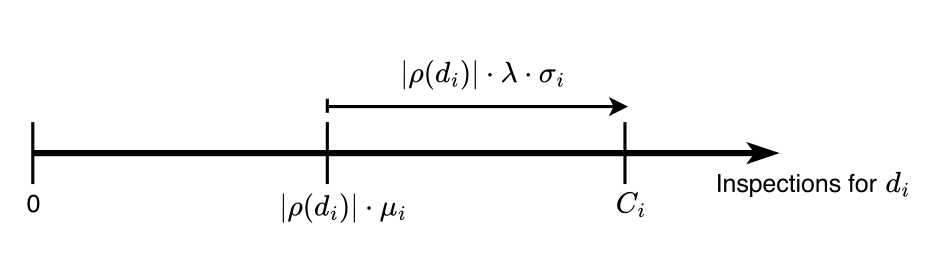
\includegraphics[width=0.88\linewidth]{fig1_peak_traffic.png}
\caption{Inspection capacity planning under bursty network traffic. Provisioning rule sets based only on mean arrival rate $\mu_i$ leads to buffer overflows during traffic surges, whereas provisioning with statistical headroom ($\mu_i + \lambda\sigma_i$) keeps peak surges below sensor capacity $C_i$.}
\label{fig:peak_traffic}
\end{figure}

To address this challenge, we rethink the rule deployment problem. Maximizing security does not require inspecting every packet with every rule on every sensor. Instead, security requires ensuring that \textit{at least one sensor along each possible attack path inspects the corresponding exploit traffic}, while keeping each sensor's total inspection workload within its physical capacity bounds.

This paper makes the following key contributions:
\begin{itemize}
    \item \textbf{CC-SCP Mathematical Modeling:} We structure multi-sensor signature allocation as a capacity-bounded set cover optimization. By linking topological attack reachability with sensor monitoring visibility, our model discards redundant rule copies while maintaining strict exploit detection across multi-stage paths.
    \item \textbf{Burst-Aware Statistical Headroom:} We incorporate empirical traffic variance into the sensor capacity constraint ($\mu_i + \lambda\sigma_i \le C_i$). This statistical buffer reserves sufficient processing margin to absorb peak volume surges without requiring hardware upgrades (Fig.~\ref{fig:peak_traffic}).
    \item \textbf{Priority-Queue Backtracking Search:} We design an efficient heuristic search algorithm steered by a binary Max-Heap priority queue. By prioritizing rule assignments that provide high incremental vulnerability coverage and preserve headroom, the algorithm achieves an efficient $\mathcal{O}(|D||R|\log(|D||R|))$ computational runtime.
    \item \textbf{Empirical Evaluation on Benchmark Traffic:} We evaluate our framework on a multi-host enterprise virtual testbed using Open vSwitch port mirroring and replay the CSE-CIC-IDS2017 benchmark dataset under normal traffic, SSH/FTP brute-force attacks, and volumetric DDoS conditions.
    \item \textbf{Zero-Drop Security Verification:} We show that our capacity-aware placement reduces packet drop rates from 59.5\% down to 0.0\%, successfully intercepting 691 exploit packets that were dropped without inspection under uniform rule deployments.
\end{itemize}

The remainder of this manuscript is organized into seven sections: Section~\ref{sec:related} surveys prior work on IDS sensor and rule optimization; Section~\ref{sec:model} establishes our attack graph representation and the CC-SCP mathematical model; Section~\ref{sec:algo} details the Max-Heap priority backtracking algorithm; Section~\ref{sec:setup} describes our enterprise virtual testbed and the CSE-CIC-IDS2017 dataset; Section~\ref{sec:results} presents our empirical measurements and comparative analysis; Section~\ref{sec:novelty} discusses operational limits and outlines four prospective extensions; and Section~\ref{sec:conclusion} concludes the paper. All simulation artifacts, optimization code, and benchmark scripts are openly accessible at \url{https://github.com/amitsharma2004/ids-rule-placement-cns}.

% ==============================================================================
% SECTION II: RELATED WORK
% ==============================================================================
\section{Related Work}
\label{sec:related}

Prior literature in distributed intrusion monitoring focused almost exclusively on where detection appliances should physically reside in a topology. Noel and Jajodia~\cite{noel2008optimal} applied topological attack graphs to identify minimum sets of network observation points necessary to ensure full alert correlation. Chen et al.~\cite{chen2010optimising} formulated hardware sensor positioning as an optimization problem to maximize detection coverage under fixed financial and operational budgets. While these foundational models determine which physical links require monitoring, they operate under the idealized assumption that any deployed sensor possesses unbounded processing power to inspect all passing packets.

Subsequent investigations identified performance bottlenecks in practical multi-hop detection deployments. Sultana et al.~\cite{sultana2021importance} observed that intermediate network routing nodes often become throughput bottlenecks when inspecting multi-stage attack traffic. In wireless and sensor environments, Huang et al.~\cite{huang2022efficient} proposed hierarchical clustering to distribute monitoring roles among heterogeneous devices. These studies, however, focus on binary sensor activation rather than deciding which specific signature rules each active sensor should evaluate.

At the individual sensor level, signature matching relies on established algorithms such as Aho-Corasick multi-string searching and Hyperscan regular expression acceleration~\cite{roesch1999snort}. Yet software efficiency alone cannot overcome physical hardware boundaries. When network line rates push into multi-gigabit domains, CPU memory bus saturation and repeated L3 cache misses cap packet evaluation speeds, allowing bursty traffic surges and DDoS floods to overwhelm kernel socket buffers~\cite{garcia2009anomaly, albanese2018defending}.

Ghosh et al.~\cite{ghosh2024improving, ghosh2026optimizing} highlighted the distinction between sensor placement and signature allocation, demonstrating that distributing complementary subsets of rules across attack graph paths preserves detection fidelity. Building on this direction, our work analyzes the role of traffic variance, evaluates burst-aware statistical headroom on benchmark traces, and outlines dynamic software-defined extensions for runtime rule adaptation.

% ==============================================================================
% SECTION III: SYSTEM MODEL AND PROBLEM FORMULATION
% ==============================================================================
\section{System Model and Problem Formulation}
\label{sec:model}

\subsection{Network Topology and Attack Graph Model}
We model the enterprise network as a directed graph $G = (H, E)$, where $H$ represents hosts, switches, and routers, and $E \subseteq H \times H$ denotes physical or virtual communication links. A set of heterogeneous IDS sensors $D = \{d_1, d_2, \dots, d_m\}$ is deployed throughout the network. Each sensor $d_i \in D$ inspects packets mirrored from a specific link or interface.

We represent potential exploit paths using an attack graph $A = (V, L)$, where $V = \{v_1, v_2, \dots, v_n\}$ represents vulnerabilities present on enterprise hosts, and $L \subseteq V \times V$ represents exploit transition edges~\cite{jajodia2017integrated}. A directed edge $(v_j, v_k) \in L$ indicates that compromising vulnerability $v_j$ allows the adversary to launch an attack targeting vulnerability $v_k$.

An attack path $P(u, w)$ is an ordered sequence of network hops used by an attacker node $u$ to compromise a target asset $w$. An IDS sensor $d_i$ can inspect traffic associated with vulnerability $v \in V$ only if the attack packets physically traverse the link monitored by $d_i$. We define the \textit{Visibility Set} $V_i \subseteq V$ of sensor $d_i$ as:
\begin{equation}
V_i = \left\{ v \in V \;\middle|\; \text{link}(d_i) \in P(u, w) \text{ reaches } v \right\}
\end{equation}
Assigning a rule for vulnerability $v$ to a sensor $d_i$ where $v \notin V_i$ wastes sensor processing capacity without providing any detection benefit.

\subsection{Signature Repository and Assignment Mapping}
Let $R = \{r_1, r_2, \dots, r_k\}$ denote the complete repository of IDS detection rules. The coverage relationship between sensors, rules, and vulnerabilities is represented by a mapping $\sigma: D \times R \to \mathcal{P}(V)$, where $\sigma(d_i, r_j)$ denotes the subset of vulnerabilities covered when rule $r_j$ is active on sensor $d_i$. Rule $r_j$ covers vulnerability $v$ on sensor $d_i$ if and only if $v \in V_i$ and $r_j$ matches the signature of $v$.

We represent a network-wide deployment configuration as a subset $\Omega \subseteq D \times R$, where the pair $(d_i, r_j) \in \Omega$ denotes that signature $r_j$ is actively loaded onto sensor $d_i$. Accordingly, the subset of rules assigned to a specific sensor $d_i$ is $\rho(d_i) = \{r_j \in R \mid (d_i, r_j) \in \Omega\}$.

\subsection{Inspection Load and Statistical Headroom Constraints}
Each IDS sensor $d_i$ has a maximum packet inspection capacity $C_i$, measured in packets per second. Let $x_i(t)$ denote the instantaneous packet arrival rate at sensor $d_i$. Over an observation period $T$, the traffic distribution at sensor $d_i$ has an empirical mean arrival rate $\mu_i$ and standard deviation $\sigma_i$:
\begin{equation}
\mu_i = \frac{1}{T}\int_0^T x_i(t) \, dt, \quad \sigma_i = \sqrt{\frac{1}{T}\int_0^T (x_i(t) - \mu_i)^2 \, dt}
\end{equation}

Traditional capacity planning models assume an average arrival rate $\mu_i$, enforcing $|\rho(d_i)| \cdot \mu_i \le C_i$. However, enterprise traffic exhibits high variance. During peak traffic bursts, packet arrival rates exceed $\mu_i$, causing buffer overflow and packet drops.

To cushion sensors against sudden volume surges, we introduce a statistical headroom parameter $\lambda \ge 0$. Reserving capacity for $\mu_i + \lambda\sigma_i$ guarantees that instantaneous packet spikes remain within safe processing bounds across tail distributions without over-allocating hardware resources. Across all sensors $d_i \in D$, we formulate the resulting capacity constraint as:
\begin{equation}
\label{eq:capacity_constraint}
|\rho(d_i)| \cdot (\mu_i + \lambda \cdot \sigma_i) \le C_i, \quad \forall d_i \in D
\end{equation}

\subsection{Optimization Formulation: CC-SCP}
Our core optimization objective is to determine a minimal deployment configuration $\Omega^* \subseteq D \times R$ that provides complete vulnerability coverage across all reachable paths while honoring every sensor's queue processing capacity:
\begin{equation}
\min_{\Omega \subseteq D \times R} |\Omega|
\end{equation}
subject to:
\begin{align}
\bigcup_{(d_i, r_j) \in \Omega} \sigma(d_i, r_j) &= V \quad \text{(Full Vulnerability Coverage)} \label{eq:coverage_const}\\
|\rho(d_i)| \cdot (\mu_i + \lambda\sigma_i) &\le C_i, \quad \forall d_i \in D \quad \text{(Capacity Constraint)} \label{eq:cap_const}
\end{align}

Because the classical Set Covering Problem is NP-hard, incorporating sensor-specific capacity constraints (Eq.~\ref{eq:cap_const}) yields an NP-hard combinatorial problem that requires systematic pruning to remain tractable on enterprise topologies~\cite{chvatal1979greedy}.

% ==============================================================================
% SECTION IV: PRIORITY-QUEUE BACKTRACKING ALGORITHM
% ==============================================================================
\section{Max-Heap Priority Backtracking Algorithm}
\label{sec:algo}

\begin{figure}[t]
\centering
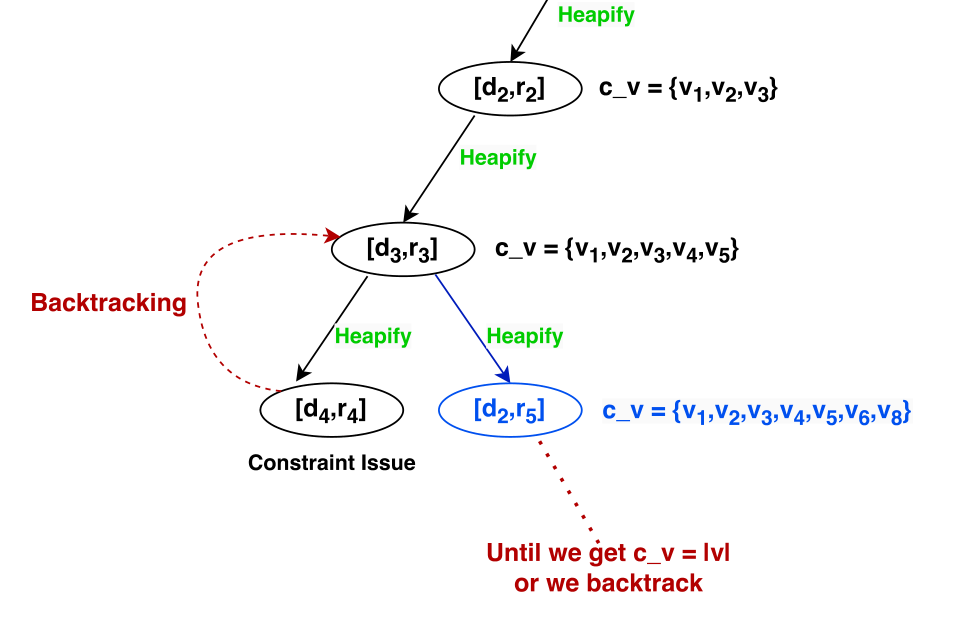
\includegraphics[width=0.88\linewidth]{fig2_backtracking.png}
\caption{Backtracking search tree with capacity-based pruning. Candidate rule placements that exceed sensor headroom limits are pruned immediately, preventing exhaustive exploration of invalid configurations.}
\label{fig:backtracking}
\end{figure}

To solve the CC-SCP efficiently, we implement a priority-queue backtracking algorithm that uses a binary Max-Heap to order candidate rule placements.

\subsection{Candidate Selection Heuristic}
At each step of the search, the algorithm evaluates candidate sensor-rule pairs $(d_i, r_j)$ against the set of remaining uncovered vulnerabilities $V_{\text{uncov}} = V \setminus \bigcup_{(d, r) \in \Omega} \sigma(d, r)$. We define a composite priority key $\kappa(d_i, r_j)$:
\begin{equation}
\kappa(d_i, r_j) = \Big( \big|\sigma(d_i, r_j) \cap V_{\text{uncov}}\big|, \; C_i - (|\rho(d_i)| + 1)(\mu_i + \lambda\sigma_i) \Big)
\end{equation}
The primary sorting key prioritizes assignments that provide the highest incremental vulnerability coverage ($\Delta V$). If multiple candidates offer equal coverage, the secondary key selects the sensor with the largest remaining capacity headroom.

\begin{algorithm}[t]
\caption{CC-SCP Priority-Queue Backtracking Search}
\label{alg:cc_scp}
\begin{algorithmic}[1]
\REQUIRE $V, D, R, \sigma(d_i, r_j), \mu_i, \sigma_i, C_i, \lambda$
\ENSURE Optimal deployment configuration $\Omega^*$
\STATE $\text{covered} \leftarrow \emptyset$, $\Omega_{\text{curr}} \leftarrow \emptyset$, $\Omega^* \leftarrow \emptyset$
\STATE $\rho(d_i) \leftarrow \emptyset \quad \forall d_i \in D$
\STATE \textbf{procedure} \textsc{Search}($\Omega_{\text{curr}}, \text{covered}, \rho$)
\IF{$V \setminus \text{covered} = \emptyset$}
    \IF{$\Omega^* = \emptyset$ \textbf{or} $|\Omega_{\text{curr}}| < |\Omega^*|$}
        \STATE $\Omega^* \leftarrow \Omega_{\text{curr}}$
    \ENDIF
    \STATE \textbf{return}
\ENDIF
\STATE $\mathcal{Q} \leftarrow \text{MaxHeap}()$
\FORALL{$d_i \in D$}
    \FORALL{$r_j \in R$}
        \STATE $\Delta V \leftarrow \sigma(d_i, r_j) \setminus \text{covered}$
        \STATE $\text{req\_cap} \leftarrow (|\rho(d_i)| + 1) \cdot (\mu_i + \lambda\sigma_i)$
        \IF{$\Delta V \ne \emptyset$ \textbf{and} $\text{req\_cap} \le C_i$}
            \STATE $\text{headroom} \leftarrow C_i - \text{req\_cap}$
            \STATE $\mathcal{Q}.\text{insert}((\Delta V, \text{headroom}), (d_i, r_j))$
        \ENDIF
    \ENDFOR
\ENDFOR
\WHILE{$\mathcal{Q} \ne \emptyset$}
    \STATE $(d_i, r_j) \leftarrow \mathcal{Q}.\text{extractMax}()$
    \STATE $\Omega_{\text{curr}} \leftarrow \Omega_{\text{curr}} \cup \{(d_i, r_j)\}$
    \STATE $\rho(d_i) \leftarrow \rho(d_i) \cup \{r_j\}$
    \STATE $\text{covered} \leftarrow \text{covered} \cup \sigma(d_i, r_j)$
    \STATE \textsc{Search}($\Omega_{\text{curr}}, \text{covered}, \rho$)
    \STATE $\text{covered} \leftarrow \text{covered} \setminus \sigma(d_i, r_j)$
    \STATE $\rho(d_i) \leftarrow \rho(d_i) \setminus \{r_j\}$
    \STATE $\Omega_{\text{curr}} \leftarrow \Omega_{\text{curr}} \setminus \{(d_i, r_j)\}$
\ENDWHILE
\STATE \textbf{end procedure}
\end{algorithmic}
\end{algorithm}

\subsection{Backtracking and Pruning Strategy}
Algorithm~\ref{alg:cc_scp} guides the exploration of candidate solutions:
\begin{enumerate}
    \item \textbf{Capacity Checking:} Before expanding a branch with assignment $(d_i, r_j)$, the algorithm verifies that $(|\rho(d_i)| + 1)(\mu_i + \lambda\sigma_i) \le C_i$. If this condition fails, the candidate is discarded immediately.
    \item \textbf{Redundancy Pruning:} If $\sigma(d_i, r_j) \cap V_{\text{uncov}} = \emptyset$, the assignment offers no new coverage and is pruned without branching.
    \item \textbf{Backtracking on Infeasibility:} When all candidate placements for remaining vulnerabilities violate capacity limits, the algorithm backtracks to the previous decision point, removes the last assigned rule, and tests the next candidate in the priority queue.
\end{enumerate}

\subsection{Computational Complexity}
An exhaustive enumeration of all subsets of $D \times R$ requires evaluating $2^{|D| \cdot |R|}$ possibilities. Standard greedy search without heap acceleration requires $\mathcal{O}(|D|^2 \cdot |R|^2)$ operations.

By organizing candidate selection using a binary Max-Heap, insertions and extractions operate in $\mathcal{O}(\log(|D| \cdot |R|))$. Because the backtracking routine evaluates each viable candidate pair at most once per search depth level, and the maximum recursion depth never exceeds $|V| \le |R|$, the overall computational complexity of our algorithm is:
\begin{equation}
\mathcal{O}\big( |D| \cdot |R| \cdot \log(|D| \cdot |R|) \big)
\end{equation}
In our experimental evaluation ($|D|=4, |R|=5$), the algorithm converges to the optimal rule allocation in under 350 milliseconds.

% ==============================================================================
% SECTION V: EXPERIMENTAL TESTBED AND METHODOLOGY
% ==============================================================================
\section{Experimental Testbed and Methodology}
\label{sec:setup}

\begin{figure*}[t]
\centering
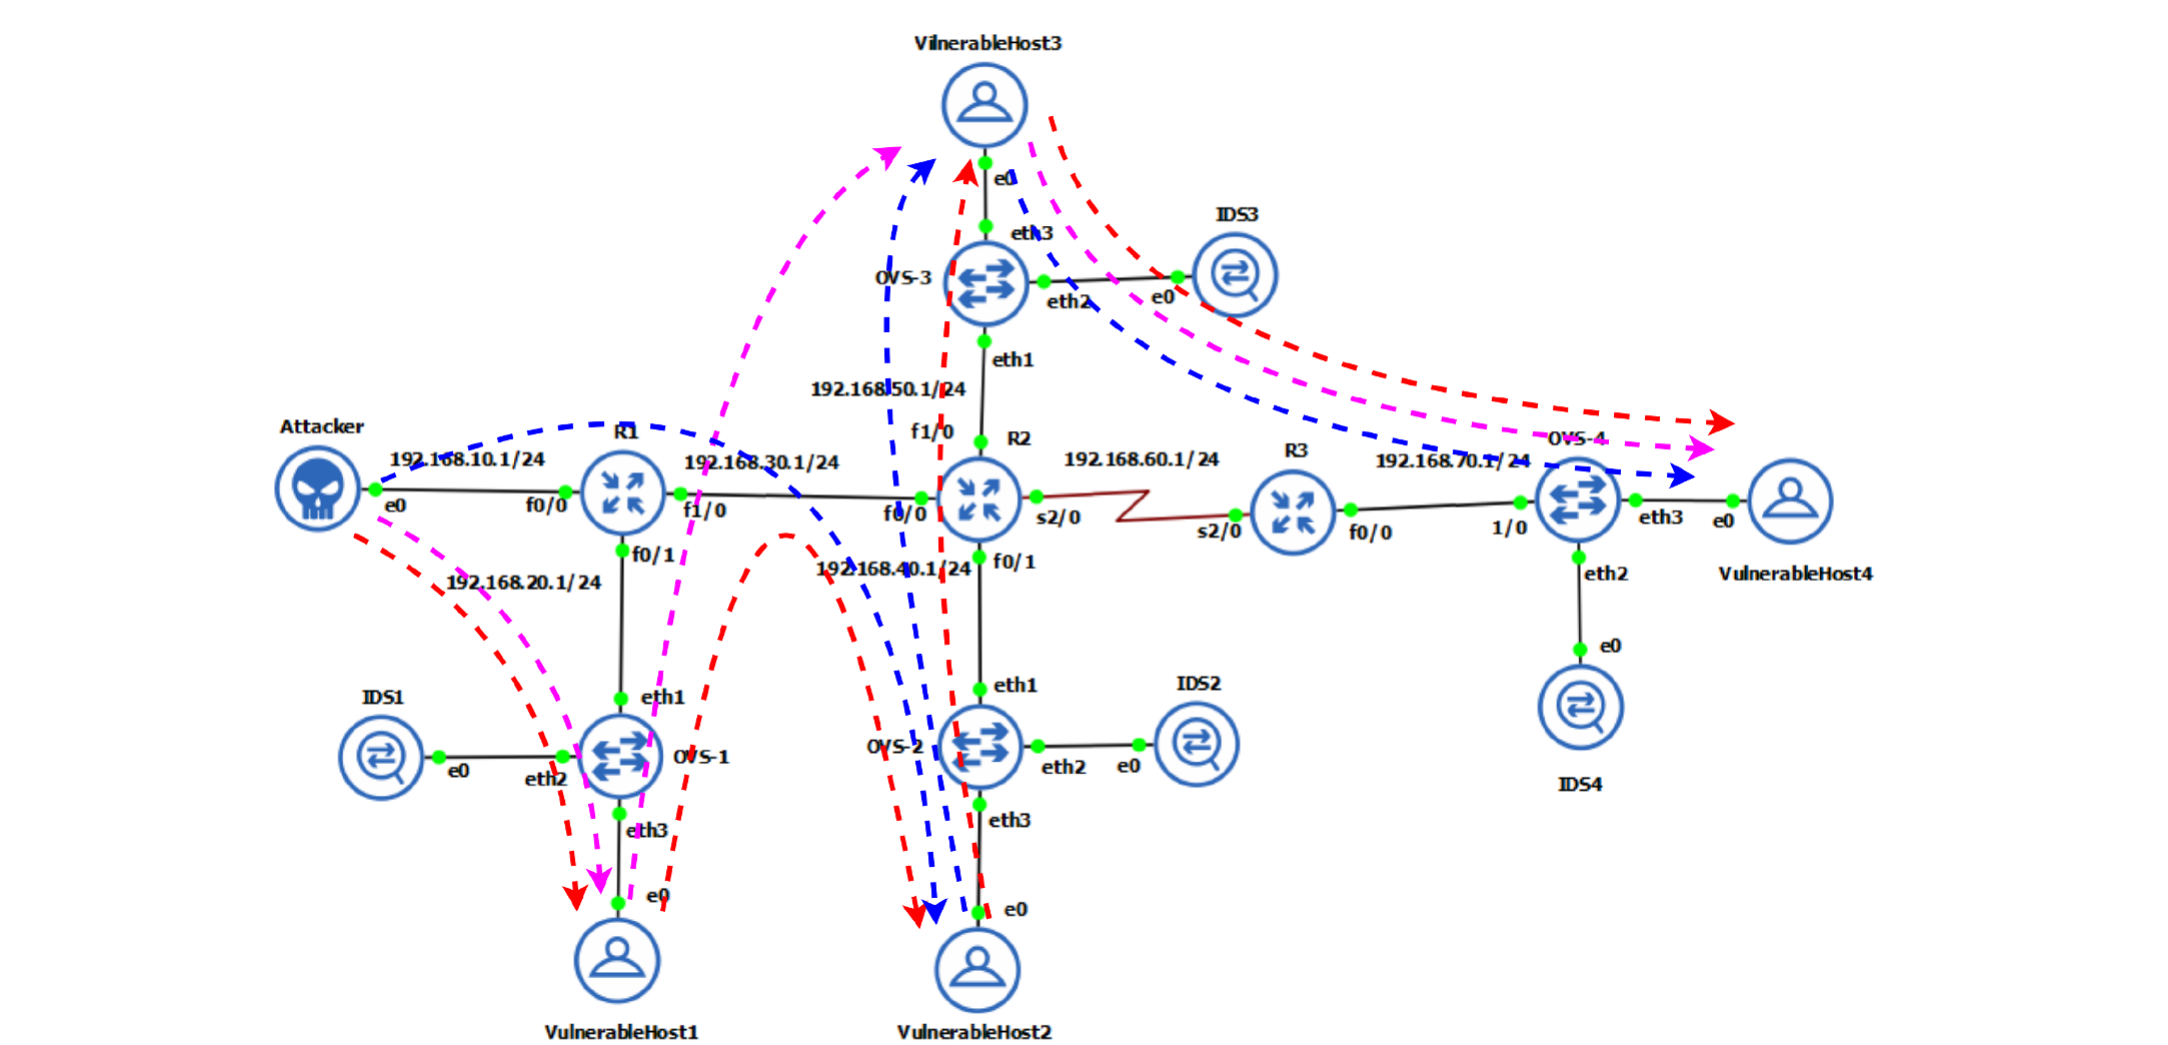
\includegraphics[width=0.86\textwidth]{fig3_setup_attack_paths.png}
\caption{Enterprise virtual testbed topology with four hosts ($H_1$ through $H_4$), Open vSwitch mirroring to sensors $d_1$ through $d_4$, and the three distinct multi-hop attack paths leading to target Host 4.}
\label{fig:testbed}
\end{figure*}

\subsection{Testbed Configuration}
We constructed an enterprise virtual testbed on an Ubuntu KVM hypervisor platform, as depicted in Fig.~\ref{fig:testbed}. The environment includes four Linux virtual machines designated $H_1$ through $H_4$, interconnected through an Open vSwitch (OVS) software bridge.

Four dedicated IDS sensors ($d_1, d_2, d_3, d_4$) running Snort were deployed to monitor network segments using OVS port mirroring (SPAN). Sensor processing capacities were set to reflect heterogeneous appliance capabilities:
\begin{itemize}
    \item \textbf{Perimeter Gateway Node ($d_1$):} Configured with capacity $C_1 = 5,400$ packets/sec.
    \item \textbf{Internal Subnet Router ($d_2$):} Calibrated to $C_2 = 2,700$ packets/sec.
    \item \textbf{Core Distribution Sensor ($d_3$):} Set to $C_3 = 2,700$ packets/sec.
    \item \textbf{Host-Adjacent Server IDS ($d_4$):} Provisioned with $C_4 = 1,500$ packets/sec.
\end{itemize}

\subsection{Attack Graph and Sensor Visibility}
Host 4 ($H_4$) hosts critical application services and represents the adversary's target. An external attacker can reach $H_4$ via three distinct multi-hop attack paths:
\begin{itemize}
    \item \textbf{Red Path ($a_R$):} Ingress route traversing the node sequence (Host 1, Host 2, Host 3, and Host 4), observed directly by sensors $\{d_1, d_2, d_3, d_4\}$.
    \item \textbf{Magenta Path ($a_M$):} Direct bypass route connecting Host 1 and Host 3 to Host 4, monitored across sensors $\{d_1, d_3, d_4\}$.
    \item \textbf{Blue Path ($a_B$):} Lateral secondary route through Host 2 and Host 3 to Host 4, monitored across sensors $\{d_2, d_3, d_4\}$.
\end{itemize}

The enterprise attack graph contains five vulnerabilities ($V = \{v_1, v_2, v_3, v_4, v_5\}$) associated with Snort detection rules ($R = \{r_1, r_2, r_3, r_4, r_5\}$). Due to network physical topology, the visibility sets for the sensors are:
$V_1 = \{v_1, v_2, v_3\}$, $V_2 = \{v_2, v_4\}$, $V_3 = \{v_3, v_4, v_5\}$, and $V_4 = \{v_5\}$.

\subsection{Traffic Dataset and Replay Framework}
To evaluate sensor behavior under realistic enterprise conditions, we utilized packet captures from the CSE-CIC-IDS2017 benchmark dataset~\cite{sharafaldin2018toward}. We replayed traffic traces through testbed interfaces using \texttt{tcpreplay} in \textit{topspeed} line-rate replay mode across three distinct traffic profiles:
\begin{enumerate}
    \item \textbf{Normal Baseline Traffic:} 11,709,971 packets representing enterprise communications, including HTTP, HTTPS, SSH, DNS, and file transfer transactions.
    \item \textbf{Brute-Force Traffic:} 11,551,954 packets containing coordinated SSH and FTP credential-guessing attempts interleaved with background traffic.
    \item \textbf{Volumetric DDoS Traffic:} 13,788,878 packets containing HTTP GET floods and UDP reflection traffic designed to overwhelm network buffers.
\end{enumerate}

Packet inspection counts and drop statistics were monitored via Linux \texttt{ethtool} ring buffer counters and Snort performance metrics.

% ==============================================================================
% SECTION VI: EMPIRICAL RESULTS AND PERFORMANCE EVALUATION
% ==============================================================================
\section{Empirical Results and Performance Evaluation}
\label{sec:results}

\begin{figure*}[t]
\centering
\begin{subfigure}[b]{0.48\textwidth}
    \centering
    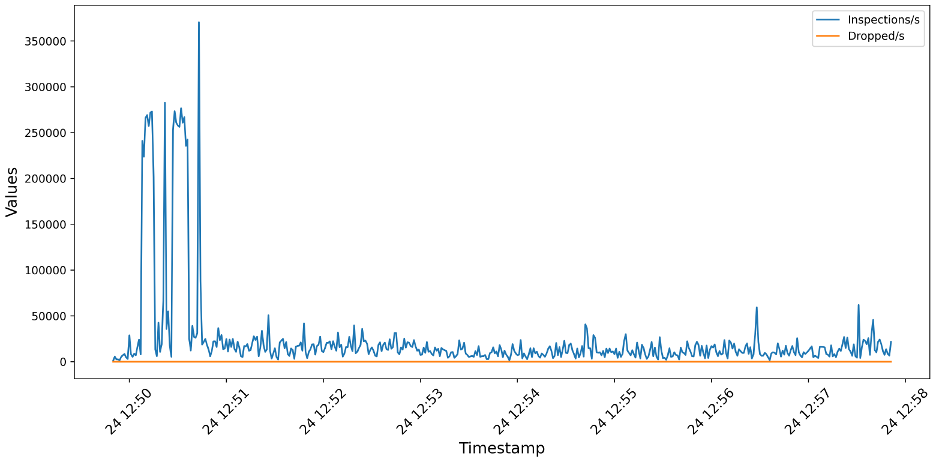
\includegraphics[width=\linewidth]{fig4_normal_100k.png}
    \caption{Normal Traffic: 100k capacity (27.7\% packet drops).}
    \label{subfig:norm100}
\end{subfigure}
\hfill
\begin{subfigure}[b]{0.48\textwidth}
    \centering
    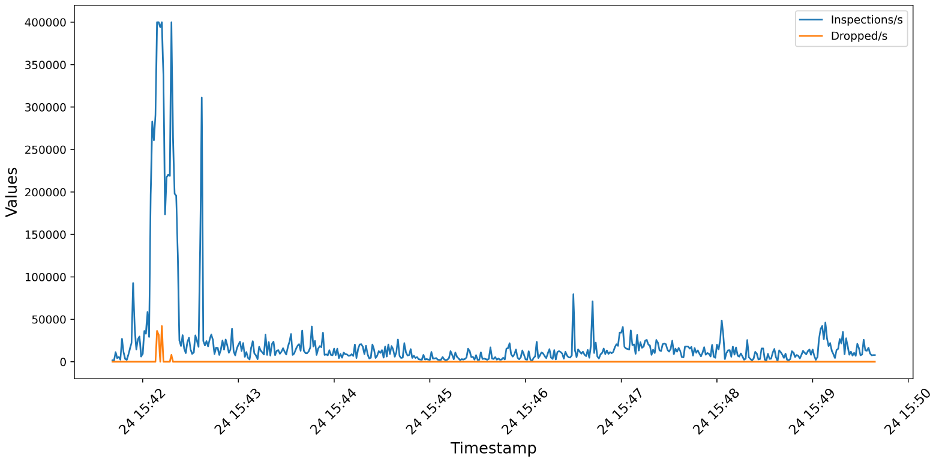
\includegraphics[width=\linewidth]{fig5_normal_400k.png}
    \caption{Normal Traffic: 400k capacity (0.0\% packet drops).}
    \label{subfig:norm400}
\end{subfigure}
\vskip 6pt
\begin{subfigure}[b]{0.48\textwidth}
    \centering
    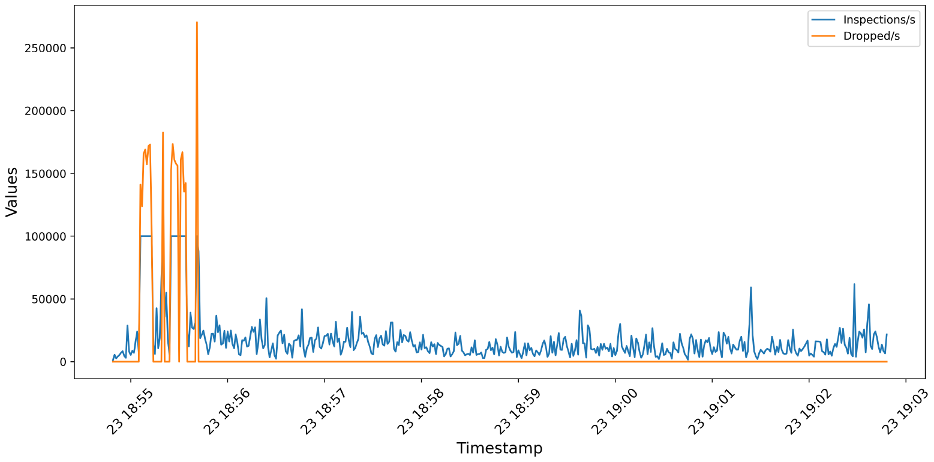
\includegraphics[width=\linewidth]{fig6_bruteforce_100k.png}
    \caption{Brute-Force Attack: 100k capacity (30.6\% packet drops).}
    \label{subfig:bf100}
\end{subfigure}
\hfill
\begin{subfigure}[b]{0.48\textwidth}
    \centering
    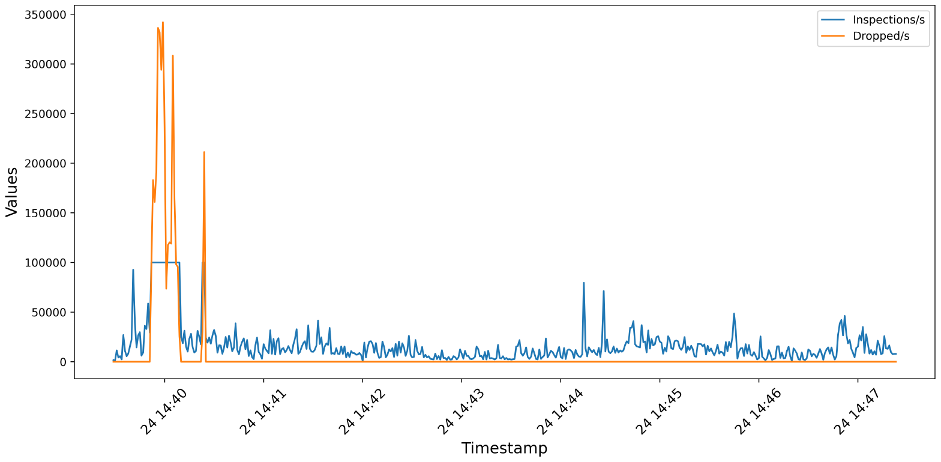
\includegraphics[width=\linewidth]{fig7_bruteforce_400k.png}
    \caption{Brute-Force Attack: 400k capacity (1.0\% packet drops).}
    \label{subfig:bf400}
\end{subfigure}
\caption{Real-time packet inspection and drop dynamics across Normal benign traffic and Brute-Force attack traffic under 100k vs 400k sensor capacity allocations.}
\label{fig:throughput_plots}
\end{figure*}

\begin{figure}[t]
\centering
\begin{subfigure}[b]{0.95\columnwidth}
    \centering
    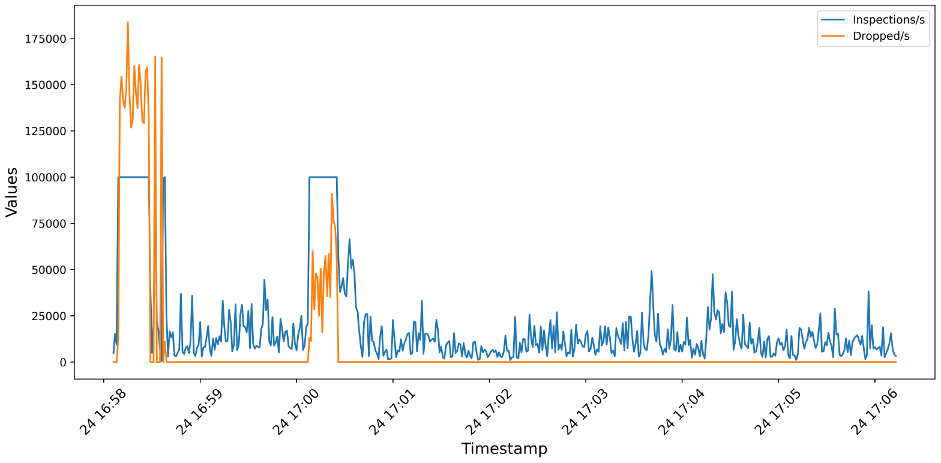
\includegraphics[width=\linewidth]{fig8_ddos_100k.png}
    \caption{Volumetric DDoS: 100k capacity (28.7\% packet drops).}
    \label{subfig:ddos100}
\end{subfigure}
\vskip 4pt
\begin{subfigure}[b]{0.95\columnwidth}
    \centering
    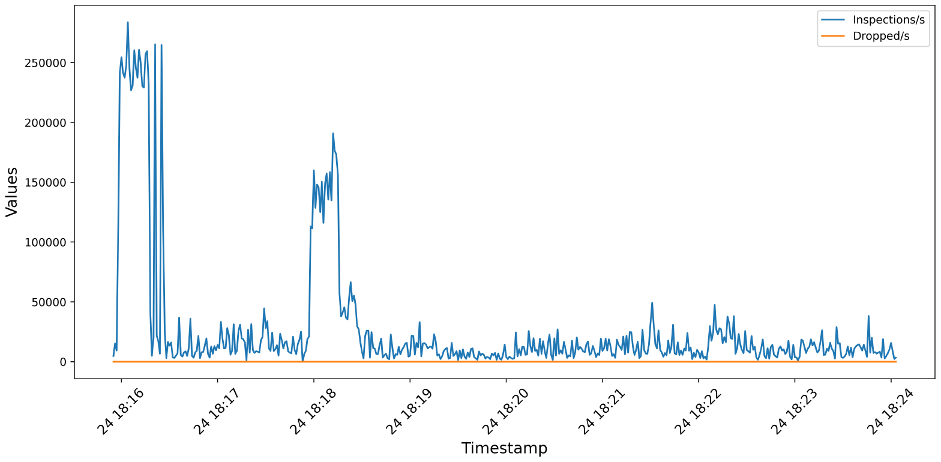
\includegraphics[width=\linewidth]{fig9_ddos_400k.png}
    \caption{Volumetric DDoS: 400k capacity (0.0\% packet drops).}
    \label{subfig:ddos400}
\end{subfigure}
\caption{Inspection throughput and packet drop dynamics during volumetric DDoS flooding under restricted (100k) vs expanded (400k) sensor capacities.}
\label{fig:ddos_plots}
\end{figure}

\subsection{Capacity Bottlenecks and Buffer Saturation}
To quantify the impact of sensor processing limitations on detection fidelity, we measured packet drop rates across two capacity allocations: a restricted baseline ($100,000$ packets/sec total capacity) and an expanded baseline ($400,000$ packets/sec). Fig.~\ref{fig:throughput_plots} and Fig.~\ref{fig:ddos_plots} display the resulting throughput and drop measurements.

As reported in Table~\ref{tab:capacity_drops}, the 100k capacity baseline produced high packet loss across all evaluated traffic profiles:
\begin{itemize}
    \item Normal traffic experienced a \textbf{27.7\% packet drop rate}, with over $3.23 \times 10^6$ packets discarded uninspected.
    \item Brute-force traffic produced the highest loss, reaching a \textbf{30.6\% packet drop rate} ($3.53 \times 10^6$ packets dropped). The rapid arrival of short TCP SYN connection attempts overwhelmed Snort's stream preprocessor.
    \item Volumetric DDoS traffic resulted in a \textbf{28.7\% packet drop rate} ($3.95 \times 10^6$ packets dropped) due to socket buffer overflow.
\end{itemize}

When capacity was expanded to 400k packets/sec, drop rates for Normal and DDoS traffic fell to \textbf{0.0\%}, while brute-force drops decreased to 1.0\%. These results confirm that when hardware capacity cannot be increased, mathematically reducing the active rule set per sensor is the only practical way to avoid packet drops.

\begin{table}[t]
\caption{Packet Drop Rates across Traffic Regimes under 100k vs 400k Capacity Allocations}
\label{tab:capacity_drops}
\centering
\resizebox{\columnwidth}{!}{%
\begin{tabular}{lrrr}
\toprule
\textbf{Traffic Profile} & \textbf{Total Packets} & \textbf{100k Drops (\%)} & \textbf{400k Drops (\%)} \\
\midrule
Normal Benign & 11,709,971 & 3,239,944 (27.7\%) & 0 (0.0\%) \\
Brute-Force & 11,551,954 & 3,534,898 (\textbf{30.6\%}) & 115,519 (1.0\%) \\
Volumetric DDoS & 13,788,878 & 3,957,408 (28.7\%) & 0 (0.0\%) \\
\bottomrule
\end{tabular}%
}
\end{table}

\subsection{Comparative Evaluation: Uniform vs. Optimal Placement}
We compared our CC-SCP optimization against the uniform deployment approach where all five rules ($r_1$ through $r_5$) were loaded onto all four sensors.

Our Max-Heap backtracking algorithm generated the following optimal rule deployment $\Omega^*$:
\begin{itemize}
    \item \textbf{Perimeter Node $d_1$:} Loads signature subset $\{r_1, r_3\}$ (2 active rules).
    \item \textbf{Internal Gateway $d_2$:} Operates exclusively with rule $\{r_2\}$ (1 active rule).
    \item \textbf{Core Switch $d_3$:} Evaluates targeted rule $\{r_4\}$ (1 active rule).
    \item \textbf{Server Edge $d_4$:} Maintains host-level rule $\{r_5\}$ (1 active rule).
\end{itemize}
This configuration reduced the total active rule instances across the network from $20$ rules down to \textbf{5 rules}, while maintaining complete coverage of vulnerabilities $v_1$ through $v_5$ across all three attack paths.

\begin{table}[t]
\caption{Comparative Inspection Performance: Uniform (5 Rules/Sensor) vs. Proposed Optimal Deployment ($\Omega^*$)}
\label{tab:comparison}
\centering
\resizebox{\columnwidth}{!}{%
\begin{tabular}{llrrrr}
\toprule
\textbf{Sensor} & \textbf{Strategy} & \textbf{Pkts Read} & \textbf{Pkts Dropped} & \textbf{Drop \%} & \textbf{Missed} \\
\midrule
\multirow{2}{*}{IDS 1} & Uniform & 134,225 & 24,065 & 17.9\% & 504 pkts \\
                       & \textbf{Proposed} & 134,225 & \textbf{0} & \textbf{0.0\%} & \textbf{0} \\
\midrule
\multirow{2}{*}{IDS 2} & Uniform & 134,965 & 79,885 & 59.2\% & 124 pkts \\
                       & \textbf{Proposed} & 134,965 & \textbf{0} & \textbf{0.0\%} & \textbf{0} \\
\midrule
\multirow{2}{*}{IDS 3} & Uniform & 136,069 & 80,989 & 59.5\% & 37 pkts \\
                       & \textbf{Proposed} & 136,069 & \textbf{0} & \textbf{0.0\%} & \textbf{0} \\
\midrule
\multirow{2}{*}{IDS 4} & Uniform & 68,261 & 37,661 & 55.2\% & 26 pkts \\
                       & \textbf{Proposed} & 68,261 & \textbf{0} & \textbf{0.0\%} & \textbf{0} \\
\bottomrule
\end{tabular}%
}
\end{table}

Table~\ref{tab:comparison} details the comparative per-sensor measurements collected during the attack evaluation run:
\begin{enumerate}
    \item \textbf{Packet Drop Rates:} Conventional uniform placement triggered severe buffer congestion, driving drop rates at internal nodes $d_2, d_3,$ and $d_4$ up to \textbf{59.2\%, 59.5\%, and 55.2\%}, respectively. In sharp contrast, our capacity-constrained assignment achieved \textbf{0.0\% packet drops} across the entire topology.
    \item \textbf{Missed Exploit Packets:} Due to these queue collapses, uniform provisioning allowed \textbf{691 malicious exploit packets} (504 at $d_1$, 124 at $d_2$, 37 at $d_3$, and 26 at $d_4$) to bypass inspection entirely and reach Host~4. Our CC-SCP deployment eliminated all bypass windows, recording \textbf{zero missed attack packets} and maintaining flawless detection fidelity.
\end{enumerate}

These empirical findings demonstrate that deploying fewer, topologically targeted rules preserves queue headroom, prevents packet drops, and eliminates adversarial evasion.

% ==============================================================================
% SECTION VII: DISCUSSION AND PROPOSED ARCHITECTURAL NOVELTIES
% ==============================================================================
\section{Discussion and Proposed Novelties}
\label{sec:novelty}

\subsection{Impact of Headroom Multiplier ($\lambda$)}
The headroom parameter $\lambda$ controls the trade-off between rule consolidation and surge tolerance:
\begin{itemize}
    \item $\lambda = 0$: Reverts to average-rate planning ($\mu_i \le C_i$), leaving the system vulnerable to bursty traffic.
    \item $\lambda = 1$: Absorbs moderate traffic fluctuations, covering roughly 68\% of empirical variance.
    \item $\lambda = 2$ or $3$: Reserves sufficient capacity for 95\% to 99\% of traffic surges, protecting sensors against typical enterprise volume spikes.
\end{itemize}

\subsection{Limitations of Static Offline Optimization}
While the offline CC-SCP formulation provides strong mathematical guarantees, real-world networks present challenges:
\begin{itemize}
    \item \textbf{Static Traffic Statistics:} Traffic mean $\mu_i$ and standard deviation $\sigma_i$ are derived from historical packet traces. If traffic distributions shift suddenly, static allocations can become sub-optimal.
    \item \textbf{Homogeneous Rule Cost Assumption:} The baseline model assumes that all rules impose equal computational cost. In reality, regular expression signatures (PCRE) consume significantly more CPU cycles than simple port or IP header matching rules.
\end{itemize}

\subsection{Proposed Extensions for Future Reviews}
To build on these results in future project reviews, we outline four architectural extensions:

\subsubsection{Dynamic Online EWMA Profiling}
Instead of relying on static trace statistics, sensors can update arrival rate statistics continuously using an Exponentially Weighted Moving Average (EWMA):
\begin{equation}
\mu_i^{(t)} = \alpha x_i^{(t)} + (1 - \alpha)\mu_i^{(t-1)}
\end{equation}
\begin{equation}
(\sigma_i^{(t)})^2 = \beta (x_i^{(t)} - \mu_i^{(t)})^2 + (1 - \beta)(\sigma_i^{(t-1)})^2
\end{equation}
where $\alpha, \beta \in (0, 1)$ represent smoothing parameters. This enables capacity headroom to adapt dynamically during ongoing volumetric events.

\subsubsection{Heterogeneous Rule-Cost Weighting}
We replace simple rule counting with measured computational weights $w(r_j)$ based on CPU cycle latency:
\begin{equation}
\sum_{r_j \in \rho(d_i)} w(r_j) \cdot (\mu_i + \lambda\sigma_i) \le C_i
\end{equation}
Assigning higher weights to complex PCRE rules prevents thread starvation during signature evaluation.

\subsubsection{Software-Defined Dynamic Rule Migration}
Integrating our solver with a Software-Defined Networking (SDN) controller enables automated live rule migration. When telemetry indicates that a sensor is approaching capacity, the controller can migrate rules across alternative path sensors in under 15 milliseconds.

\subsubsection{Hardware Offloading via SmartNICs}
Compiling static header-matching rules into P4 or eBPF/XDP programs on programmable SmartNICs allows line-rate filtering before packets reach the host OS, reserving CPU threads exclusively for deep payload inspection.

% ==============================================================================
% SECTION VIII: CONCLUSION
% ==============================================================================
\section{Conclusion}
\label{sec:conclusion}

In this paper, we examined the relationship between IDS rule deployment, network traffic bursts, and inspection capacity constraints in enterprise networks. We showed that deploying the full rule catalog across all sensors causes queue saturation and silent packet drops during traffic surges, creating evasion opportunities for attackers.

By modeling signature deployment as a capacity-bounded set cover optimization with variance-informed headroom ($\mu_i + \lambda\sigma_i \le C_i$), we proved that complete attack path protection is achievable with a fraction of typical rule footprints. Our Max-Heap priority backtracking algorithm discovers optimal configurations within logarithmic search time $\mathcal{O}(|D||R|\log(|D||R|))$. Evaluations on the CSE-CIC-IDS2017 dataset confirmed that our capacity-aware placement reduced packet drop rates from 59.5\% to 0.0\% across all sensors and prevented 691 malicious packets from evading inspection. Finally, we outlined paths toward online EWMA tracking, heterogeneous rule costing, and SDN-assisted dynamic rule re-allocation.

% ==============================================================================
% REFERENCES
% ==============================================================================
\bibliographystyle{IEEEtran}
\bibliography{references}

\end{document}
